\begin{figure}
    \centering
    \begin{tikzpicture}

\node<1>[inner sep=0pt] (motherboard) at (3,0)
    {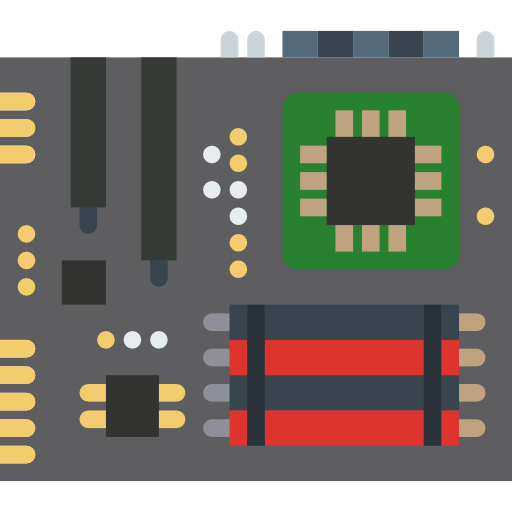
\includegraphics[width=.12\textwidth]{Simulation_sayem/pictures/motherboard.png}};
\node<2>[inner sep=0pt] (motherboard) at (3,0)
    {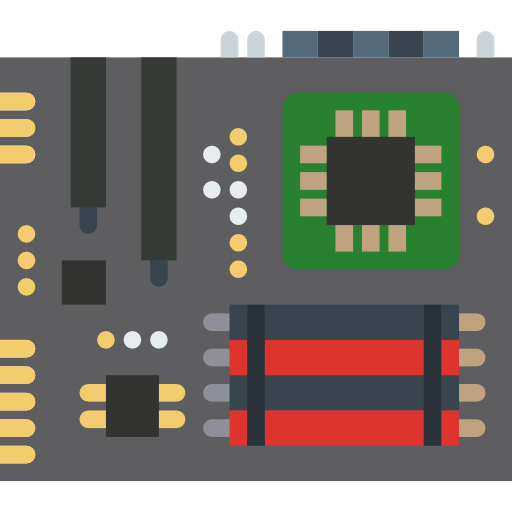
\includegraphics[width=.14\textwidth]{Simulation_sayem/pictures/motherboard.png}};
    
    
\node[inner sep=0pt] (videocard) at (6,-3)
    {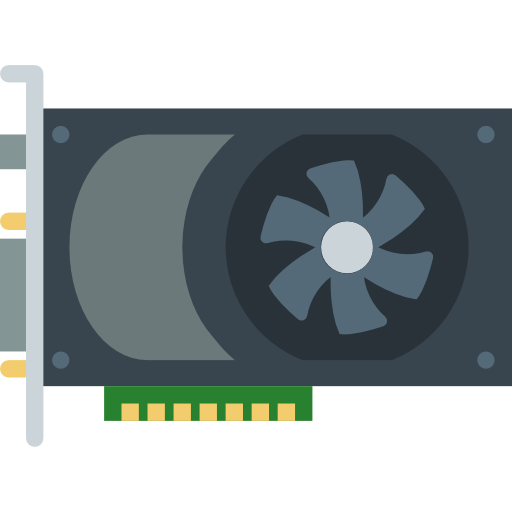
\includegraphics[width=.12\textwidth]{Simulation_sayem/pictures/video-card.png}};


\node[inner sep=0pt] (memory) at (0,0)
    {
\includegraphics[width=.12\textwidth]{Simulation_sayem/pictures/memory.png}};
\node[inner sep=0pt] (casing) at (10,1)
    {
\includegraphics[width=.12\textwidth]{Simulation_sayem/pictures/casing.jpg}};
\node[inner sep=0pt] (PSU) at (9,-2)
    {
\includegraphics[width=.12\textwidth]{Simulation_sayem/pictures/powerSupply.jpg}};


\node[inner sep=0pt] (CPU) at (6,3)
    {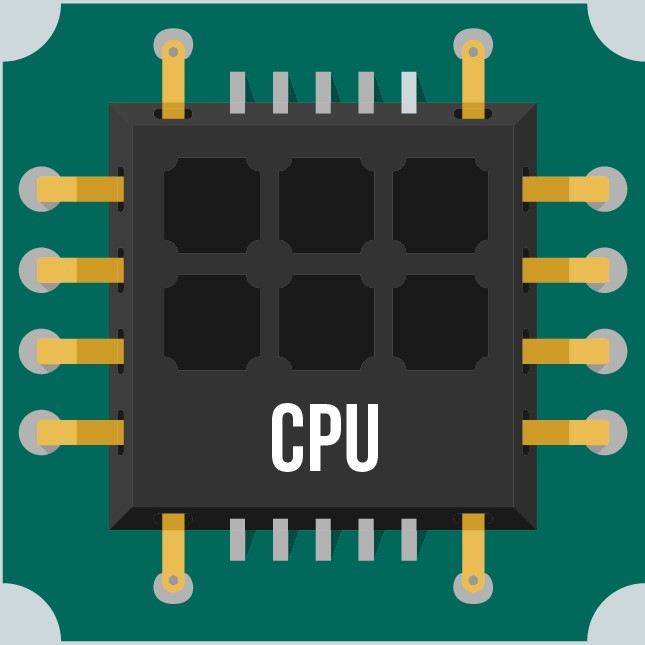
\includegraphics[width=.14\textwidth]{Simulation_sayem/pictures/processor.jpg}};
    
\draw<1-> [inactive edge] (videocard) --(PSU);
\draw<1-> [inactive edge] (motherboard) --(videocard);
\draw<1-> [inactive edge] (CPU) --(videocard);
\draw<2> [active edge] (motherboard) --(CPU);

\end{tikzpicture}
\end{figure}
